% ============================================================
% 分片：s03b  对应原文 PDF 第 37--40 页
% 负责章节：§3.1.3 The secondary product（并含 §3.1.2 落在第 37 页的末尾段落）
% 译者：translator-06   审校状态：初稿
% ============================================================

% [跨页接续: 原文第 36 页/37 页。本分片自第 37 页首词起，承接 s03a 在第 36 页末的句子
%  "the two topological twists of 3d N=4 theories are called the A and B twists with"。
%  同时说明：第 37 页上半仍属 §3.1.2（其正文越出第 36 页），按页界由本分片收录，s03a 应止于第 36 页末。]

% ==== 原文 PDF 第 37 页 ====
扭变超荷例如为 $Q_A = Q_+^{+\dot{+}} + Q_-^{-\dot{+}}$ 与 $Q_B = Q_+^{+\dot{+}} + Q_-^{+\dot{-}}$。\footnote{事实上，超荷 $Q_H = Q_+^{+\dot{+}}$ 本身即幂零，并引出一个全纯--拓扑混合的扭变，其类比对象是 2.1.1 节所述二维 $\mathcal{N}=(2,2)$ 的半扭变超荷 $Q_H = \bar Q_+$。}
% [原文疑误: 脚注 34 中 "leads to a mixed holomorphic-topological," 之后缺中心名词（按上下文应为 twist），译文补足为“全纯--拓扑混合的扭变”；不改动其后的类比关系。]

局域算子的 $Q_B$ 上同调与 $Q_A$ 上同调给出两类受保护算子的环；在三维 $\mathcal{N}=4$ 情形下，这些局域算子分别实现真空模空间的（超凯勒）希格斯分支（Higgs branch）与库仑分支（Coulomb branch）上全纯函数所成的代数。与标准二维 $\mathcal{N}=(2,2)$ 理论的手征环完全类似，标准三维 $\mathcal{N}=4$ 规范理论的希格斯分支手征环不受任何量子修正。另一方面，库仑分支与库仑分支手征环，类比于由扭手征环参数化的 $A$ 模型的凯勒模空间，会受到大量非微扰修正。尽管如此，它近来已获得完整的数学定义 [66, 67]。这些局域算子的后代张成相应模空间的切丛。\footnote{我们要指出：即使像本文这样只关注对拓扑环（它们刻画真空流形的几何）敏感的扭变，在更一般的语境中也会遇到延展的（而非局域的）BPS 算子（例如 [68]）。}\footnote{所谓“标准”，指的是超多重态与 $\mathcal{N}=4$ 矢量多重态极小耦合的三维 $\mathcal{N}=4$ 理论。与二维情形相同，上述镜像自同构意味着存在这些多重态的扭变版本，可用于构造 $\mathcal{N}=4$ 理论。为简单起见，我们还限制在超多重态按余切型 $T^*R := R \oplus \bar R$ 的线性表示变换的情形，其中 $R$ 是规范群的酉表示，$\bar R$ 为其复共轭表示。}

存在一种（红外的）三维对偶，称为三维镜像对称（3d mirror symmetry），以区别于通常的镜像对称概念；它把两个 $\mathcal{N}=4$ 理论 $\mathcal{T}_{3d} \leftrightarrow \tilde{\mathcal{T}}_{3d}$ 联系起来，其方式是通过上述三维 $\mathcal{N}=4$ 代数的镜像自同构来交织超对称的作用。特别地，它把 $\mathcal{T}_{3d}$ 的库仑分支与镜像理论 $\tilde{\mathcal{T}}_{3d}$ 的希格斯分支等同起来（反之亦然）[69]。与通常的镜像对称一样，这一对偶往往将近乎经典的对象（希格斯分支）与高度量子的对象（库仑分支）互换。这一三维场论对偶享有漂亮的弦论 [70, 71] 与 M 理论 [72] 提升。

\subsubsection{次级乘积}

上文已经看到，拓扑后代包含 $d$ 维拓扑扭变理论中局域算子关联函数的位置依赖信息——可以用它们在不同算子构型之间构造显式的同伦。$Q$-闭局域算子关联函数的位置无关性（在上同调意义下）意味着：局域算子的碰撞在这样一个扭变理论的局域算子 $Q$-上同调上诱导出一种代数结构。给定两个 $Q$-闭局域算子 $O_1$、$O_2$，其乘积是另一个 $Q$-闭局域算子，它由把 $O_1$ 放在 $x_1$、把 $O_2$ 放在 $x_2\neq x_1$ 处、然后取极限 $x_1\to x_2$ 得到（至多相差 $Q$-恰当项）。换一种说法，该乘积由把两个互不相交的开 $d$-球包含进一个更大的开 $d$-球所诱导；对应乘积 $(O_1O_2)O_3$ 的图示见 Figure 8。

需要注意的是，我们同样可以按任意顺序碰撞，至多相差 $Q$-恰当项。具体而言，正如 2.3 节对 $d=2$ 情形的简述，给定 Figure 8 中的三个局域算子，我们也可以先将 $O_2$ 与 $O_3$ 碰撞，再把所得结果与 $O_1$ 碰撞，得到局域算子 $O_1(O_2O_3)$。至多相差 $Q$-恰当项，这两个算子必须相同，即 $(O_1O_2)O_3 - O_1(O_2O_3) = Q(\ldots)$，这意味着碰撞赋予局域算子的 $Q$-上同调
% ==== 原文 PDF 第 38 页 ====
以结合代数的结构。更一般地，$Q$-闭局域算子的碰撞在同伦意义下是结合的；3.2 节将回到这些同伦。

\begin{figure}[tbp]
  \centering
  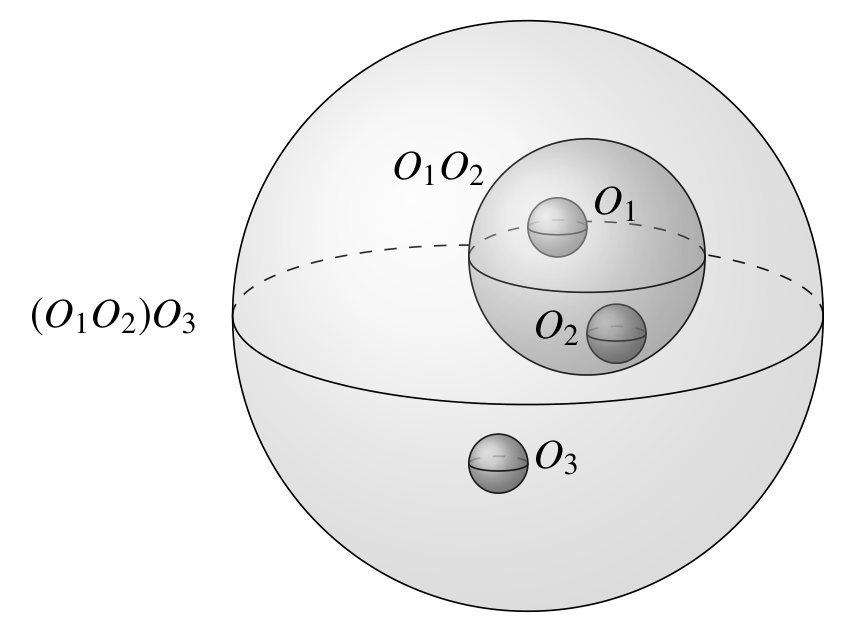
\includegraphics[width=0.62\linewidth]{figures/fig08.png}
  \caption{$d$ 维 TQFT 中由三个小球包含进两个较大的球所诱导的迭代乘积 $(O_1O_2)O_3$ 的图示。（原文第 38 页，Figure 8）}
\end{figure}

当 $d\ge 2$ 时，$\mathbb{R}^d$ 中两个不同点（更确切地说，开球）的任意构型都可以连续形变为任何其他构型，因此 $d\ge 2$ 时局域算子的 $Q$-上同调必然是交换（结合）代数。另一方面，在 $d=1$ 时，无法把 $x_2<x_1$ 的构型连续形变为 $x_1<x_2$ 的构型，因此存在两种未必相等的可能碰撞。于是，$d=1$ 时局域算子的 $Q$-上同调具有未必交换的结合代数结构。

尽管 $d\ge 2$ 时局域算子的 $Q$-上同调是交换的，拓扑下降却会在局域算子的 $Q$-上同调上额外诱导出所谓的次级乘积（secondary product）。本小节沿用 [73, 74] 的表述回顾这一思想。对 $Q$-闭局域算子 $O_1$ 与 $O_2$，次级乘积 $\{O_1,O_2\}$ 定义为：把 $O_2$ 置于 $x_2$，再把 $(d-1)$-形式算子 $O_1^{(d-1)}$ 在环绕 $x_2$ 的 $(d-1)$-球面 $S^{d-1}$ 上积分：
% [Tutor Note: 度数记账：$O_1^{(d-1)}$ 是 $O_1$ 的 $(d-1)$-形式后代；把 $(d-1)$-形式沿 $(d-1)$ 维球面积分后回到 0 形式。故次级乘积使总次数降低 $d-1$，诱导出的泊松括号次数为 $1-d \bmod 2$（碰撞乘积的次数为 0）。]
\begin{equation}\tag{3.9}
\{O_1,O_2\} = \int_{S^{d-1}_{x_2}} O_1^{(d-1)}\, O_2(x_2).
\end{equation}

这是一个局域算子，因为它支在一个足够大的单个球内部；它仍是 $Q$-闭的，因此可以再次看作代表一个 $Q$-上同调类。

更一般地，考虑 $\mathbb{R}^d$ 上两个点（更确切地说，小开圆盘）的构型空间，记作 $C_{\mathbb{R}^d}(2)$；拓扑下降允许对该构型空间的每个同调类 $H_\bullet(C_{\mathbb{R}^d}(2))$ 定义一个“乘积”，参见 [55, Section 1.3] 与 [73, Section 3.2.1]。给定一个 $n$ 维链 $\Gamma$，定义次数为 $-n$ 的乘积 $\star_\Gamma(O_1,O_2)$ 为
\begin{equation}\tag{3.10}
\star_\Gamma(O_1,O_2) = \int_\Gamma (O_1(x_1)O_2(x_2))^{(n)},
\end{equation}
其中我们在由 $\Gamma$ 确定的构型空间上对第 $n$ 个后代积分。对 Stokes 定理与下降方程的一次快速应用给出\footnote{若 $\Gamma$ 是 $n$ 维链，则“沿 $\Gamma$ 积分形式”这一运算，即 $\omega \mapsto \int_\Gamma \omega$，在把总次数（含形式次数）的宇称与费米子宇称同等看待时，自然是次数为 $-n$ 的映射。由于 $Q$ 的次数为 1，把 $Q$ 移过积分 $\int_\Gamma$ 时便产生因子 $(-1)^n$。}
% ==== 原文 PDF 第 39 页 ====
% [Tutor Note: (3.11) 中两处符号的来源：其一，$Q$ 为 1 次算子，穿过 $-n$ 次的积分映射 $\int_\Gamma$ 时产生 $(-1)^n$；其二，下降方程把 $d(O_1O_2)^{(n-1)}$ 改写为 $Q$ 的变分，再用 Stokes 定理把 $\int_\Gamma d(\cdot)$ 化为边界项 $\int_{\partial\Gamma}$，即得第二行三项。]
\begin{equation}\tag{3.11}
\begin{aligned}
Q(\star_\Gamma(O_1,O_2))
&= (-1)^n \int_\Gamma \left( d(O_1O_2)^{(n-1)} + \left( (QO_1)O_2 + (-1)^{F(O_1)}O_1(QO_2) \right) \right)\\
&= (-1)^n \left( \star_{\partial\Gamma}(O_1,O_2) + \star_\Gamma(QO_1,O_2) + (-1)^{F(O_1)} \star_\Gamma(O_1,QO_2) \right).
\end{aligned}
\end{equation}

特别地，若 $\Gamma$ 是闭链且 $O_1$、$O_2$ 是 $Q$-闭的，则乘积 $\star_\Gamma(O_1,O_2)$ 也是 $Q$-闭的。此外，若两条链 $\Gamma$、$\Gamma'$ 同调，即 $\Gamma' = \Gamma + \partial\Gamma''$，其中 $\Gamma''$ 为某个 $n+1$ 维链，则（在 $Q$-闭局域算子上）这两个乘积相差 $Q(\star_{\Gamma''}(O_1,O_2))$，因而在 $Q$-上同调层面一致。

构型空间 $C_{\mathbb{R}^d}(2)$ 同伦等价于 $(d-1)$-球面 $S^{d-1}$，其同调有一个 0 次生成元，对应通常的碰撞乘积 $(O_1,O_2)\mapsto O_1O_2$，以及一个 $(d-1)$ 次生成元，对应次级乘积 $(O_1,O_2)\mapsto \{O_1,O_2\}$。\footnote{当 $d=1$ 时，球面 $S^{d-1}$ 是两点 $[1]$、$[-1]$ 的简单集合，相应的乘积为映射 $(O_1,O_2)\to O_1O_2$ 与 $(O_1,O_2)\to (-1)^{F(O_1)F(O_2)}O_2O_1$；最高维闭链的类比物是这两点的形式差 $[S^0] = [+1]-[-1]$，于是次级乘积的类比物就是通常的分次对易子
\[
\star_{[S^0]}(O_1,O_2) = O_1O_2 - (-1)^{F(O_1)F(O_2)}O_2O_1 .
\]
该现象与三维 TQFT 中次级乘积经由 $\Omega$-背景的量子化有关，参见 [73, Section 6]。更确切地说，开启 $\Omega$-背景要求考虑构型空间 $C_{\mathbb{R}^3}(2)\sim S^2$ 的 $U(1)$-等变同调（关于 $\mathbb{R}^3$ 中绕固定轴的旋转）。它由不动点／极点 $[N]\sim[1]$、$[S]\sim[-1]$ 生成（作为等变参数 $\epsilon$ 及其逆 $\epsilon^{-1}$ 的多项式环）；由 $[N]$ 与 $[S]$ 诱导的乘积同次级乘积之间的关系，恰好相当于泊松括号与分次对易子之间的关系
\[
[N]-[S] = \epsilon[S^2] \leftrightarrow \star_{[N]}(O_1,O_2) - \star_{[S]}(O_1,O_2) = \epsilon \star_{S^2}(O_1,O_2) .
\]}
% [存疑: 脚注 38 原文作 "the sphere $S^{d-1}$ is a simply pair of points"，语序应为 "is simply a pair of points"，译文按后者理解。]
% [Tutor Note: 脚注中 $d=1$ 的对应关系值得记住：$S^0=[+1]-[-1]$ 对应分次对易子；开启 $\Omega$-背景后 $[N]-[S]=\epsilon[S^2]$ 对应泊松括号与分次对易子之差，这是三维 TQFT 中次级乘积“量子化”的几何来源。]
由于该构型空间没有其他同调类，它们就是上同调层面仅有的两种“乘积”。（下一节还会用到这些构型空间上更一般的链，而不只是闭链。）与碰撞乘积一起，次级乘积赋予局域算子的 $Q$-上同调以 $\mathbb{Z}/2\mathbb{Z}$-分次泊松代数的结构，其泊松括号的次数为 $1-d \bmod 2$。（在许多带有给出费米子数的 $U(1)$ $R$ 对称性的例子中，它可以提升为 $\mathbb{Z}$-分次代数，正如前面关于扭变的讨论。）

下面看一个用于说明的简单例子，其细节见 [73, Section 4]。
% [背景补充: 多重矢量场（polyvector fields）是 $\wedge^p T^{(1,0)}X$ 的截面，其取值可有 $(p,q)$ 双次数；$B$ 模型的局域算子在几何上正是这类对象，其上的 Schouten--Nijenhuis 括号是向量场 Lie 括号的分次推广。]
考虑靶空间为某个 Calabi--Yau 流形 $X$ 的二维 $B$ 模型，世界面取平坦。前面已经推断，局域算子的空间同构于 $X$ 上多重矢量场（polyvector fields）的 Dolbeault 上同调。换言之，$Q$-上同调同构于取值于全纯切丛任意外幂 $\wedge^p(T^{(1,0)}X)$ 的 $(0,q)$-形式的 $\bar\partial_X$-上同调。手征环元素是 $X$ 上的全纯函数，即上同调的 0 次部分。与 $A$ 模型不同，$B$ 模型不受任何瞬子修正，因此初级乘积就是
% ==== 原文 PDF 第 40 页 ====
上同调上通常的几何楔积，参见 2.3.2 节：
\begin{equation}\tag{3.12}
[O_1]\cdot[O_2] = [O_1\wedge O_2].
\end{equation}
% [Tutor Note: 物理图像：$B$ 模型的多重矢量场即 $\wedge^p T^{(1,0)}X$ 的截面，初级乘积正是其楔积，完全经典、不受世界面瞬子修正；这正是 $B$ 模型与 $A$ 模型（量子上同调）的关键差别，也是 $B$ 模型能纯代数地处理的原因。]

这一情形的次级乘积在弦论及其他语境中相当著名，称为 Gerstenhaber 括号。用几何语言说，它称为多重矢量场的 Schouten--Nijenhuis 括号，是通常矢量场上 Lie 括号的推广。为简单起见，设靶空间为 $X=\mathbb{C}^N$。扭变超荷为 $Q = Q_B := \bar Q_+ + \bar Q_-$，而按先前的记号，“矢量”超荷可由分量为 $-\frac{1}{2i}Q_-$、$\frac{1}{2i}Q_+$ 的矢量给出。在平坦的 $\mathbb{C}^N$ 上，多重矢量场由全纯函数 $f(\phi)$ 与全纯矢量场 $g^n(\phi)\partial_{\phi^n}$ 生成。我们仍把（费米子的）坐标矢量场记作 $\bar\zeta_n := \partial_{\phi^n}$。为得到次级括号 $\{\bar\zeta_n,\phi^m\}$，需要 $\bar\zeta_n$ 的单形式后代：
% [Tutor Note: 易错预警：此处的 $\star$ 是 Hodge 星算子，与乘积符号 $\star_\Gamma$ 无关，切勿混淆。(3.13) 中的 $Q_\mu$ 是“矢量”超荷的分量 $\left(-\frac{1}{2i}Q_-,\frac{1}{2i}Q_+\right)$，$[Q_\mu,\cdot]$ 即沿该分量作拓扑下降。]
\begin{equation}\tag{3.13}
\bar\zeta_n^{(1)} = -dx^\mu[Q_\mu,\bar\zeta_n] = -(\star d\bar\phi_n).
\end{equation}

这里 $d$ 仍为 de Rham 微分，$\star$ 为 Hodge 星算子。还可注意到 $d\bar\zeta_n^{(1)} = d\star d\bar\phi_n = \frac{\delta S}{\delta\phi^n}$，因而与 $\phi^n$ 的运动方程成正比。若把它当作算子，Euclidean QFT 的标准论证表明 $\frac{\delta S}{\delta\phi}(z,\bar z)$ 在接触项之外为零，于是在任何关联函数中，算子乘积 $\frac{\delta S}{\delta\phi}(z,\bar z)\phi(w,\bar w)$ 等价于插入一个 delta 函数二形式 $\delta^2(z-w,\bar z-\bar w)$（前提是二者各自与关联函数中其他算子分离）。这可以直接由分部积分证明：
\begin{equation}\tag{3.14}
\begin{aligned}
&\int \mathcal{D}\phi\,\mathcal{D}\bar\phi\; e^{-S}\frac{\delta S}{\delta\phi}(z,\bar z)\phi(w,\bar w)\\
&\quad = \int \mathcal{D}\phi\,\mathcal{D}\bar\phi \left( -\frac{\delta}{\delta\phi(z,\bar z)}\left( \phi(w,\bar w)e^{-S} \right) + \delta^2(z-w,\bar z-\bar w)e^{-S} \right)\\
&\quad = \int \mathcal{D}\phi\,\mathcal{D}\bar\phi\; \delta^2(z-w,\bar z-\bar w)e^{-S}.
\end{aligned}
\end{equation}

按次级括号的定义，有
\begin{equation}\tag{3.15}
\begin{aligned}
\{\bar\zeta_n,\phi^m\} &= \left[ \oint_{S^1_{w,\bar w}} \bar\zeta_n^{(1)} \phi^m(w,\bar w) \right]\\
&= \left[ \int_{D^2_{w,\bar w}} d\bar\zeta_n^{(1)} \phi^m(w,\bar w) \right],
\end{aligned}
\end{equation}
其中我们用方括号表示上同调类，第二行用了 Stokes 定理。利用刚才得到的结果并把 delta 函数二形式代入最后一行，得到
\begin{equation}\tag{3.16}
\{\bar\zeta_n,\phi^m\} = \delta_n^m .
\end{equation}
% [Tutor Note: (3.15) 到 (3.16) 的关键一步：由 (3.13) 与 (3.14)，$d\bar\zeta_n^{(1)}$ 在无接触项时为零；Stokes 定理把 $S^1$ 上的积分改写为 $D^2$ 上 $d\bar\zeta_n^{(1)}$ 的积分，非零结果完全来自接触项 $\delta^2(z-w,\bar z-\bar w)$，故得到 $\delta_n^m$。]

也可以通过对方程 $\phi^m$ 作下降来得到这一结果，这是检验答案的有益方式。类似的计算表明，两个 $\phi$ 之间或两个 $\bar\zeta$ 之间的次级括号为零，原因在于这些算子之间缺乏接触项以及由此得出的运动方程。可以验证，这一次级括号（至多相差一个费米子宇称因子 $\{a,b\}_{SN} = (-1)^{F(a)-1}\{a,b\}$）就是多重矢量场上的几何 Schouten--Nijenhuis 括号，并且它特别满足如下性质：（分次的）反对称性、对每个自变量都是（分次的）导子、以及（分次的）Jacobi 恒等式。
